	Idea Intuitiva: variable que toma valores con determinada ``regla de probabilidad''.\\
	Nos interesa hacer una descripci\'on matem\'atica de fen\'omenos no deterministas (inciertos). Por lo que necesitamos entonces mediciones cuantitativas.\\
	Una variable aleatoria toma valores en los\'umeros reales.

	\subsection{Variables Aleatorias}
		\begin{itemize}
			\item Mapeo de Resultados:\\
				Como una idea m\'as formal, usaremos variables aleatorias X para mapear resultados de un espacio muestral a n\'umeros reales $X: \Omega \leftarrow R$.\\
				No siempre se mapean resultados elementales a n\'umeros. Muchas veces se mapean eventos no at\'omicos a un mismo n\'umero.\\
				En general, nos interesar\'a ser\'a determinar la ``ley de probabilidad'' que rige el comportamiento de la variable aleatoria que estamos estudiando: con qu\'e probabilidad observamos ciertos valores.
			\item Definici\'on:
                             Sea $(\Omega,\ C,\ P)$ un espacio de probabilidad y $(R,\ \beta)$ un espacio de medida definido sobre los reales $(R)$. Una variable aleatoria se define como una funci\'on $X: \Omega \leftarrow R$ tal que para todo $B$ en $\beta$, su pre-imagen $X^{-1}(B)$ est\'a en $C$.
			\item Requerimientos de la Colecci\'on de eventos medibles:
			\begin{enumerate}
				\item no vac\'ia
				\item cerrada bajo complementos
				\item cerrada bajo uniones numerables
			\end{enumerate}
			\item Sigma-\'algebra de Borel ($\beta$):\\
				Queremos poder medir la probabilidad de que la variable aleatoria tome valores en intervalos [a, b].\\
				Incluimos primero todos los intervalos de la forma $(-\infty, x]$ con x en R.\\
  				Cerramos finalmente la familia bajo complementos y uniones numerables.
			\item Probabilidad Inducida: La propiedad que le pedimos a las variable aleatorias permite medir probabilidades en R.\\
				Para todo $B$ en la sigma-\'algebra $\beta$: $$P(B)\ :=\ P(w\ :\ X(w)\ esta\ en\ B)\ =\ P(X^{-1}(b))$$ \\
				S\'olo gracias a que $X^{-1}(b)$ es medible en el espacio de probabilidad original podemos calcular esta probabilidad!
		\end{itemize}
	\subsection{Funci\'on de Distribuci\'on}
		\begin{itemize}
			\item Definici\'on:\\
                         	La distribuci\'on asociada a una variable aleatoria X se define como la funci\'on F: R \-> [0,1] $$ F(x)\ =\ P((-\infty, x])$$
			\item M\'etodo:\\
				Existen dos metodos, el facil y poco-practico:
				\begin{enumerate}
					\item Determinar el subconjunto de valores de $\Omega$ mapeados a esos valores de R.
					\item Calcular la probabilidad de ese conjunto de valores de $\Omega$.
				\end{enumerate}
				Y el que si hay que seguir, en el cual la idea es caracterizar la probabilidad de los eventos que generan la sigma \'algebra en $R: (-\infty, x]$.\\
				Descomponemos en eventos para los que conocemos la probabilidad:
				$$(-4,5]\ =\ (-\infty,\ 5] - (-\infty,\ 4]$$
				$$P(-4,5]\ =\ P(-\infty,\ 5] - P(-\infty,\ 4]$$
				$$P(-4,5]\ =\ F(5)\ -\ F(4)$$

			\item Variables Discretas:
				En este caso, existen ``intervalos de probabilidad'' para cada punto, describiendo saltos por cada $X=x_n$.\\
					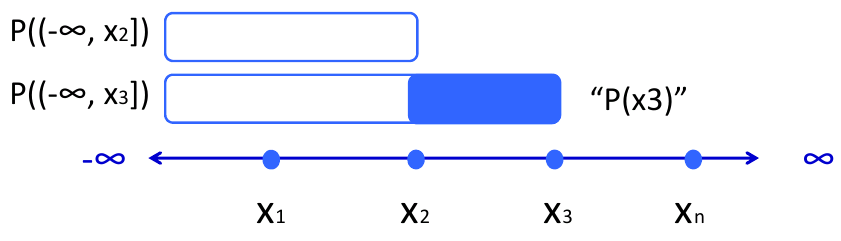
\includegraphics[height=3.5cm]{images/cap7-discretas.png}\\
				$$\therefore\ P(X=x_n)\ =\ F(x_n)\ -\ F(x_{n-1})$$
			\item Variables Continuas: No podemos ver el problema por intervalos definidos, ya que cada itervalo posee infinitos puntos. Se utiliza el concepto de densidad de Probabilidad.
				
		\end{itemize}
	\subsection{Funci\'on de Probabilidad o Cuant\'ia}
		\begin{itemize}
			\item Definici\'on
                           La funci\'on de probabilidad o cuant\'ia asociada a una variable aleatoria discreta se define como la funci\'on $p: S* \leftarrow [0,1]$ 
				$$p(x_0)\ =\ p(-\infty)$$
				$$p(x_n)\ =\ F(x_n)\ -\ F(x_n-1)$$\\
				 S es el conjunto de valores que toma X (soporte de la distribuci\'on).

			\item M\'etodo: Para calcular la probabilidad de cualquier evento A medible en R.
				$$P(A)\ =\ \int_{A}p(x_i)dx\ =\ \sum_{x_i\ \varepsilon\ A}p(x_i)$$
			\item Propiedades que se deben cumplir
				$$1\ =\ P(R)\ =\ \sum_{x_i\ \varepsilon\ R}p(x_i)$$
				$$1\ =\ \sum_{i}^{n}p(x_i)$$
			\item Densidad de Probabilidad (para variables continuas)\\
				Si existe una funci\'on p(x) tal que para todo evento A en los reales, se verifica:
				$$P(A)\ =\ \int_{A}p(x)dx$$\\
				En donde $p(x)$ se denomina funci\'on de densidad de probabilidad y X se dice absolutamente continua.
				\begin{itemize}
					\item Probabilidad de un evento en particular:
						$$F(x)\ =\ \int_{-\infty}^{x}p(x)dx$$
				\end{itemize}

		\end{itemize}
